\section{Introducción}
El formato de archivos de audio digital wav (o wave), es un formato sin compresión de datos que fue desarrollado por Microsoft e IBM, es utilizado para almacenar sonidos en una computadora. Admite archivos mono y estéreos (un canal o dos respectivamente) a diversas resoluciones y velocidades de muestreo.\\ Debido a que no presenta pérdida de calidad, es comúnmente usado profesionalmente para guardar audio en CDs o DVDs. Pero tiene como desventaja, que los archivos creados bajo este formato son bastante grandes en comparación con otros formatos comprimidos como mp3 u ogg.\\ El formato de archivos wav es una variante del formato RIFF (formato de archivo para el intercambio de recursos). Un archivo en formato RIFF, empieza con una cabecera de archivo (file header) seguida de una secuencia de fragmentos de datos (data chunks). Un archivo wav comúnmente, es solo un archivo RIFF pero con una sola ''wave'' chunk, la cual esta formada por dos sub-chunks (fmt sub-chunk y data sub-chunk). A esta forma se le conoce como la forma ''canónica'' de un archivo en formato wav.\\
A continuación se presenta una lista con todos los campos que almacenan la información dentro del archivo wav:
\begin{itemize}
	\item ChunkID (4 bytes): Contiene las letras ''RIFF'' en ascii.
	\item ChunkSize (4 bytes): Es el tamaño del archivo entero menos los 8 bytes de los campos anteriores que no son contados.
	\item Format (4 bytes): Contiene las letras ''WAVE''.
	\item Subchunk1ID (4 bytes): Contiene las letras ''fmt''.
	\item Subchunk1Size (4 bytes): Contiene el tamaño del resto del subchunk que queda a partir de este número.
	\item AudioFormat (2 bytes): Regularmente almacena el número 1, si se guarda algún otro número este indica algún tipo de compresión.
	\item NumChannels (2 bytes): 1 para mono, 2 para stereo.
	\item SampleRate (4 bytes): La frecuencia de muestreo que se uso para muestrear el archivo (8000, 44100, etc).
	\item ByteRate (4 bytes): Es igual a: SampleRate*NumChannels*BitsPerSample/8.
	\item BlockAlign (2 bytes): Guarda el número de bytes por cada muestra (considerando todos los canales). Se obtiene mediante: NumChannels*BitsPerSample/8.
	\item BitsPerSampl (2 bytes): La cantidad de bits que se almacenan por muestra (8 bits, 16 bits, etc).
	\item SubChunk2ID (4 bytes): Contiene las letras ''data''.
	\item SubChunk2Size (4 bytes): Es el número de bytes de los datos, también puede considerarse como el resto del subchunk apartir de este dato.
	\item Data (tamaño del SubChunk2Size): Son los datos del sonido almacenado. 
\end{itemize}
Los campos ChunkID, ChunkSize y Format componen la cabecera del archivo. Los campos Subchunk1ID, Subchunk1Size, AudioFormat, NumChannels, SampleRate, ByteRate, BlockAlign y BitsPerSample componen el primer sub-chunk llamado fmt. Los campos Subchunk2ID, Subchunk2Size y data componen el segundo sub-chunk llamado data.\\ La figura 1 muestra de forma gráfica las cabeceras y campos antes descritos:
\begin{figure}[H]
	\centering
	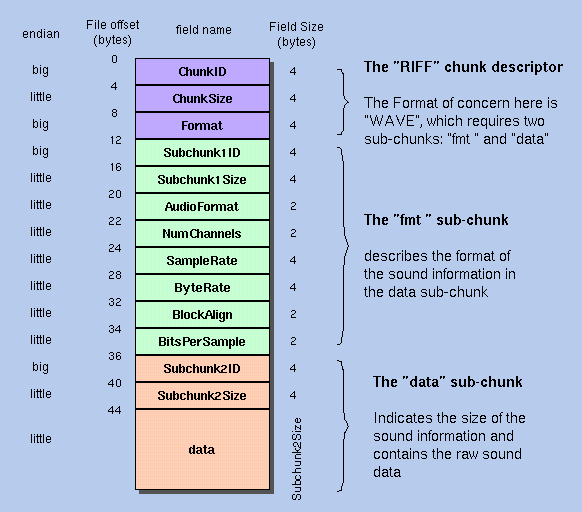
\includegraphics[scale=.7]{img/cabeceras.png}
	\caption{Campos que componen un archivo canónico wav}
	\label{fig:cabeceras}		
\end{figure}
